% 05-wavefunctions — figs 2-6 reproduced under the two-row protocol + fig 22
\section{Wave functions and structure functions}
\label{sec:wavefunctions}

Every figure in this section follows one protocol.  The top row recomputes
the 1990 figure at its original parameters, with the published curves
overlaid as digitized markers; where the original left a parameter
unstated, the caption cites the recovered value.  The bottom row repeats
the measurement at 2026 resolutions.  Nothing in the top rows is fit or
tuned: the markers ring our points where the two agree, and stand apart
where they do not.

\begin{figure*}
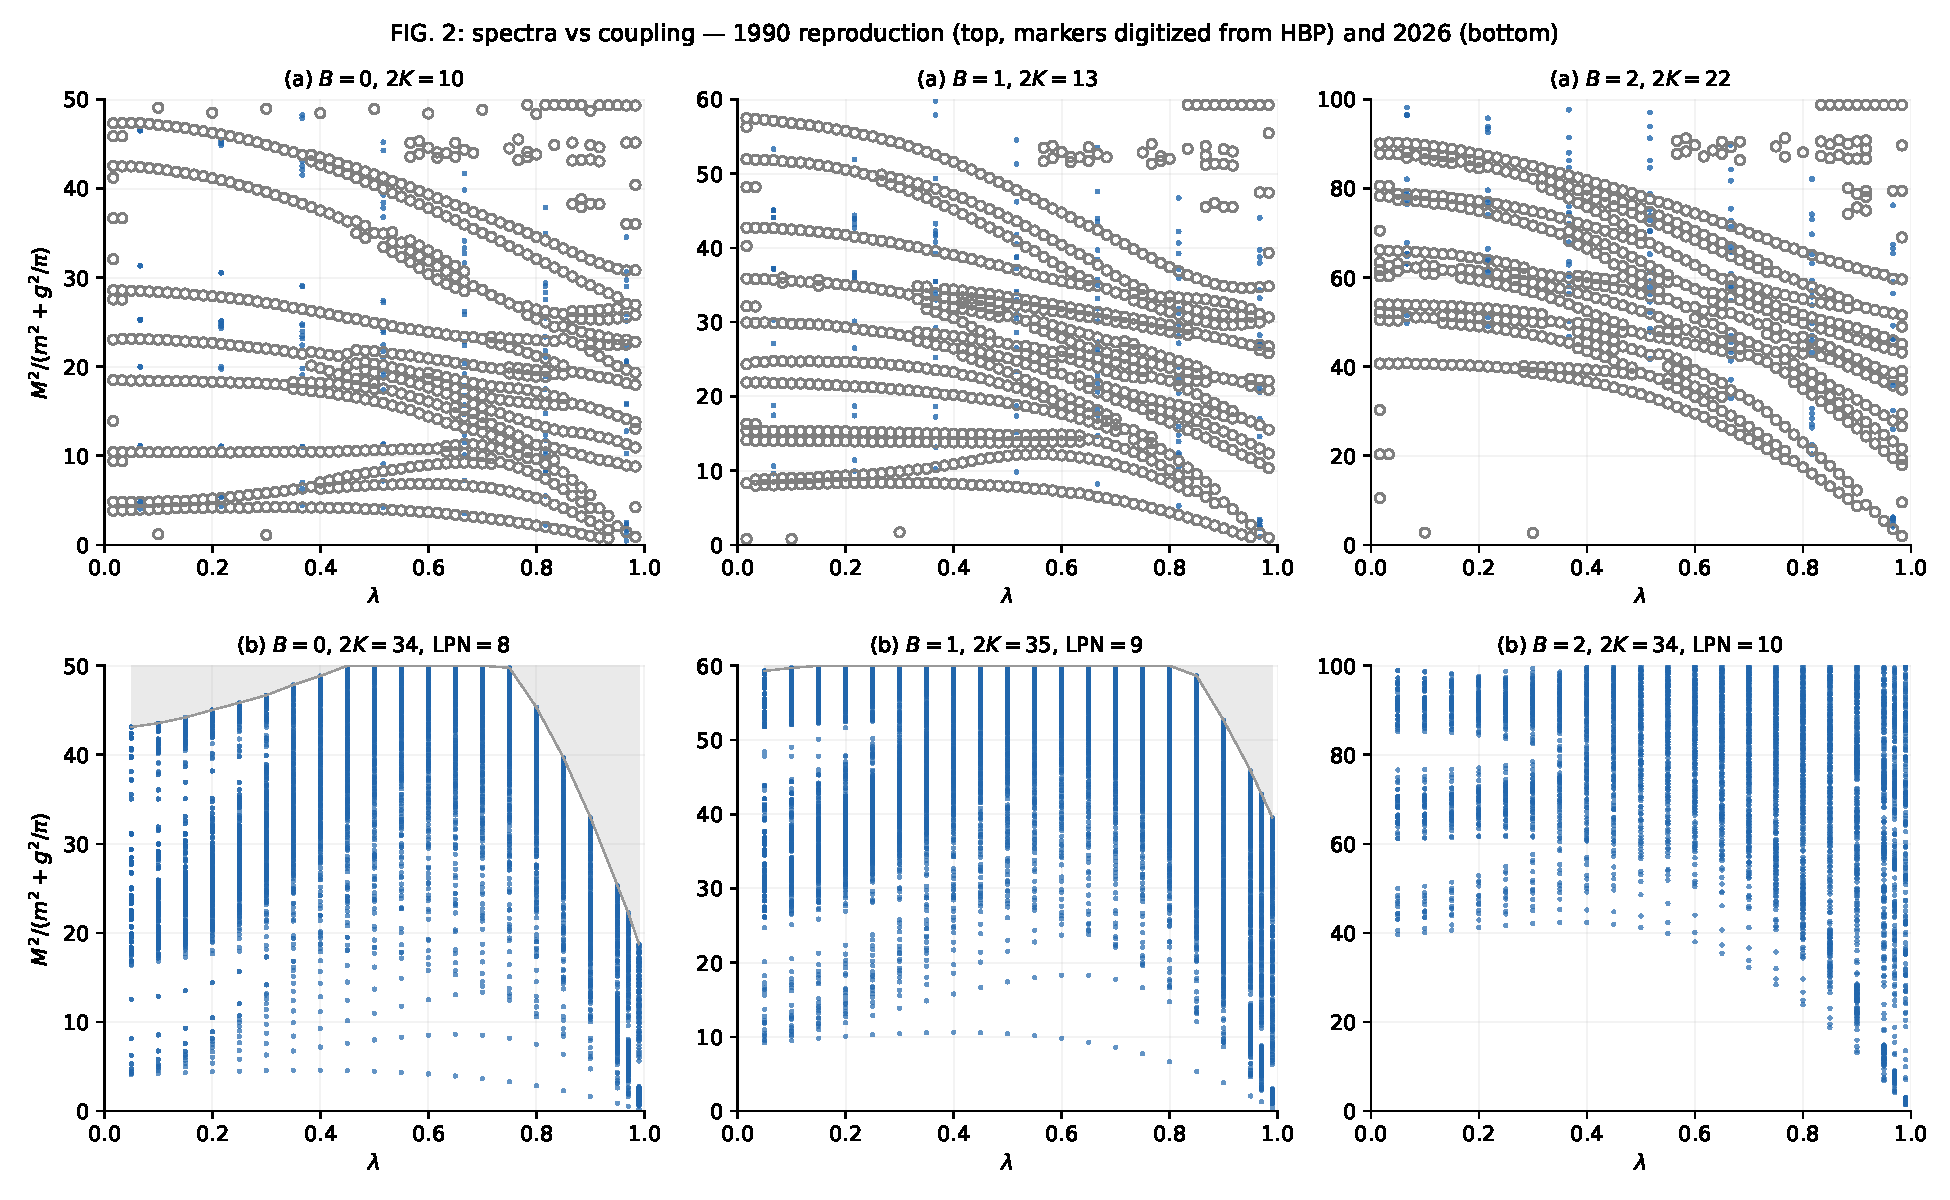
\includegraphics[width=\textwidth]{figs/fig2_spectra.pdf}
\caption{Spectra against the coupling $\lambda = [1+\pi m^2/g^2]^{-1/2}$,
$N=3$, all Hamiltonians standard, no fits.  Top: $B=0,1,2$ at
$2K = 10, 13, 22$, untruncated, markers digitized from Fig.~2 of
Ref.~\cite{Hornbostel:1988fb} (panel-to-$B$ assignment recovered; the
original caption omits it).  Bottom: $2K = 34, 35, 34$ at Fock truncation
$\mathrm{LPN} = 8, 9, 10$, lowest 250--400 states; the gray region marks
$M^2$ above the highest computed level, where states exist but are not
computed.}
\label{fig:spectra}
\end{figure*}

Figure~\ref{fig:spectra} is the coarsest and most complete comparison: the
full spectrum, scattering states included, across the coupling.  At the
1990 resolutions our levels sit inside the digitized markers across all
three baryon sectors.  At $2K = 34$ the same panels fill in: the level
density grows roughly linearly with $K$, isolated bound states remain
visible under the multi-hadron bands, and every level flows to zero at the
chiral point as Sec.~\ref{sec:massless} requires.  A resolution lesson
surfaced in drafting this panel and is worth recording.  At small
$\lambda$ a state of $L$ partons sits near $M^2/(m^2+g^2/\pi) \approx
L^2$, so matching the untruncated 1990 window requires Fock depth, not
resolution; a first attempt at $2K = 50$ with $\mathrm{LPN} = 6$ was
missing the entire upper half of the original panel, structurally.

\begin{figure}
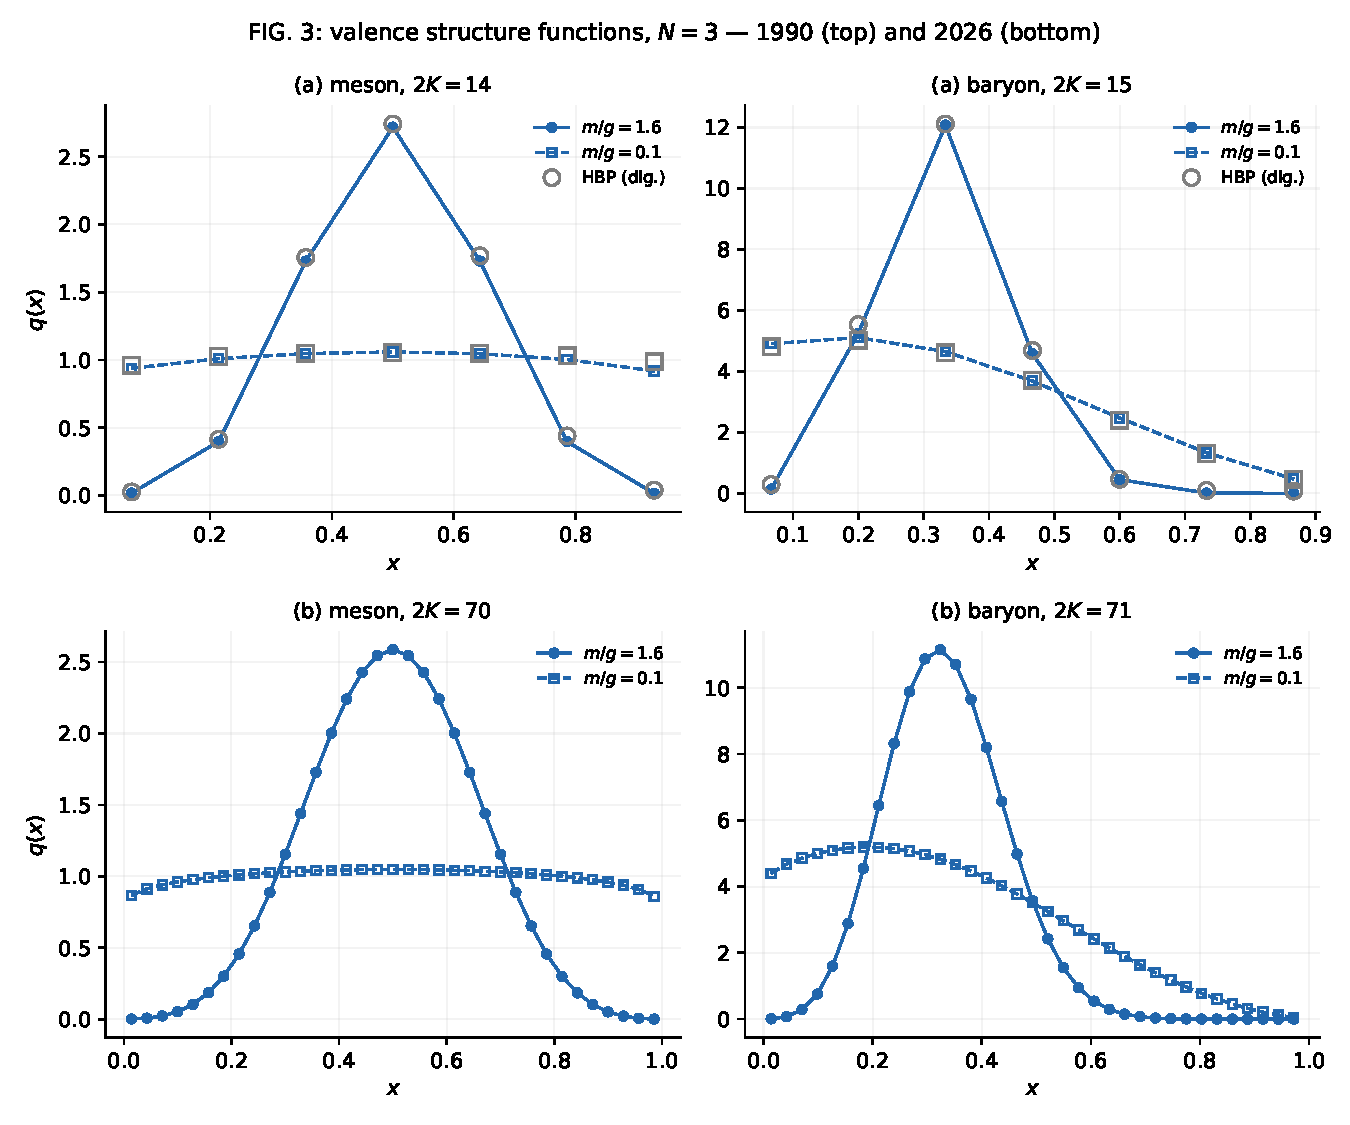
\includegraphics[width=\columnwidth]{figs/fig3_valence.pdf}
\caption{Valence structure functions, $N=3$, $m/g = 1.6$ (filled) and
$0.1$ (open), standard Hamiltonian, ground states, no fits.  Top:
$2K = 14$ (meson) and $15$ (baryon), the values recovered for the 1990
figure, whose caption omits them; markers digitized from Fig.~3 of
Ref.~\cite{Hornbostel:1988fb}.  Bottom: $2K = 70$ and $71$ at
$\mathrm{LPN} = 4$ and $5$.}
\label{fig:valence}
\end{figure}

The valence structure functions (Fig.~\ref{fig:valence}) repeat the
pattern.  At the recovered 1990 resolutions the digitized markers ring our
points; at $2K = 70$ the same curves are smooth.  The physics is as the
original described: weak coupling peaks the meson near $x = 1/2$ and the
baryon near $1/N$, and strong coupling flattens both toward the massless
distributions of Sec.~\ref{sec:massless}.

% \itodo{Fig. 4 (higher-Fock structure functions incl. qbar and the pion
% content of the baryon) needs its 2026 runs at both couplings — add to
% phase4a_config and draft the paragraph here.}

\begin{figure*}
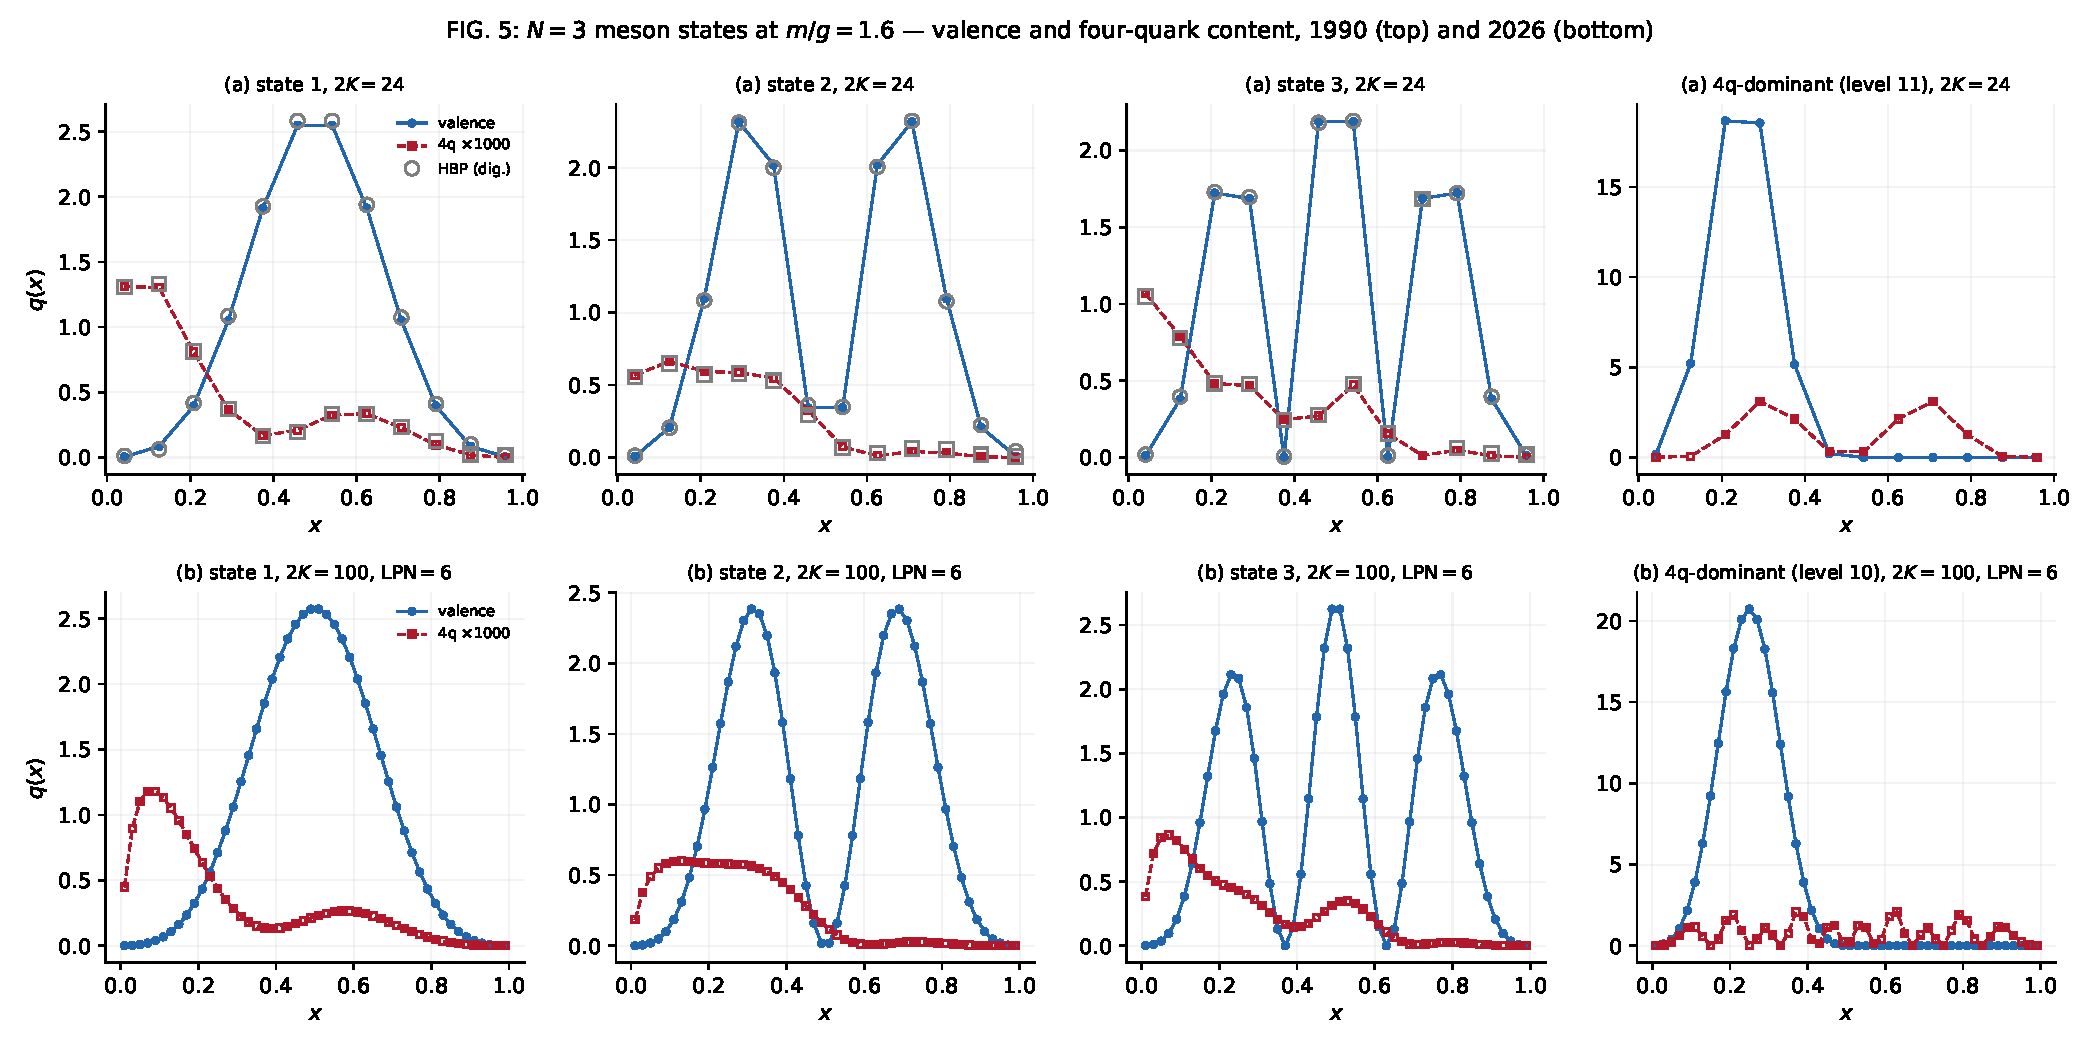
\includegraphics[width=\textwidth]{figs/fig5_meson_wf.pdf}
\caption{$N=3$ meson states at $m/g = 1.6$, standard Hamiltonian: valence
(solid) and four-quark (dashed, scaled by the stated multiplier) content.
Top: $2K = 24$, untruncated, markers digitized from Fig.~5 of
Ref.~\cite{Hornbostel:1988fb}; the last panel's digitized markers are
withheld because that panel of the original carries a second axis and the
traces calibrate to it.  Bottom: $2K = 60$, $\mathrm{LPN} = 6$, lowest 40
states.  The last column selects the first state whose four-quark Fock
weight exceeds one half, rather than a fixed level number.}
\label{fig:mesonwf}
\end{figure*}

The meson excitations (Fig.~\ref{fig:mesonwf}) add a selection question
the 1990 paper answered by inspection.  Its Fig.~5(d) showed ``the
eleventh state,'' identified in the text as two $q\bar q$ pairs in the
$\pi\pi$ continuum.  We select that physics directly: the last column
shows the first state whose four-quark Fock weight exceeds one half,
computed from the block-diagonal norm (Sec.~\ref{sec:exotics}).  At
$2K = 24$ the selector lands on level 11 --- the 1990 identification,
recovered independently.  At $2K = 60$ it lands on level 12, and the
four-quark profile peaks near $x = 1/4$: two pairs, each near half the
momentum, as the continuum interpretation requires.

\begin{figure*}
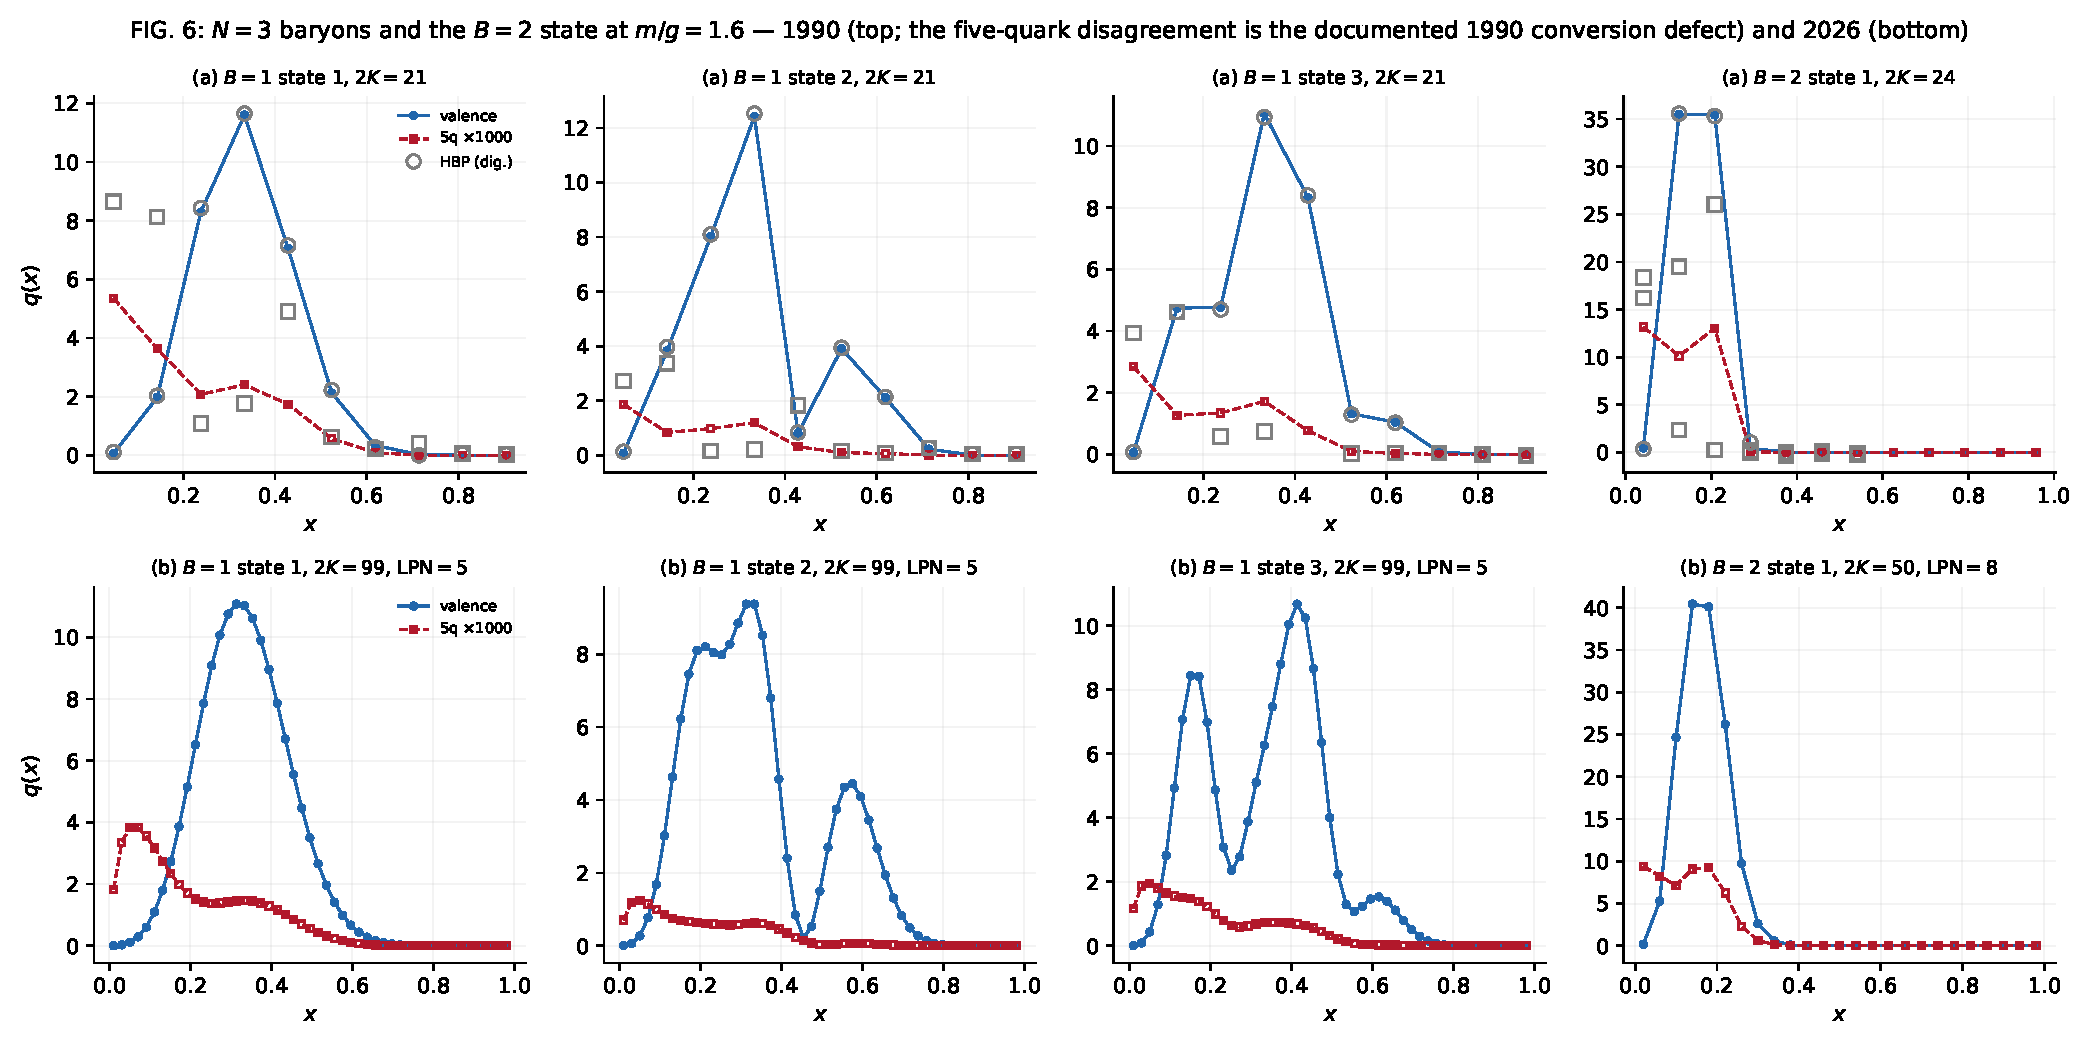
\includegraphics[width=\textwidth]{figs/fig6_baryon_wf.pdf}
\caption{$N=3$ baryon states and the $B=2$ state at $m/g = 1.6$, standard
Hamiltonian: valence (solid) and five- or eight-parton (dashed, scaled)
content.  Top: $2K = 21$ ($B=1$) and $24$ ($B=2$, a value the 1990
caption omits), untruncated, markers digitized from Fig.~6 of
Ref.~\cite{Hornbostel:1988fb}.  Bottom: $2K = 69$ and $50$ at
$\mathrm{LPN} = 5$ and $8$.  The five-quark disagreement in the first
three top panels is deliberate; see text.}
\label{fig:baryonwf}
\end{figure*}

Figure~\ref{fig:baryonwf} contains the one part of the 1990 paper we can
reproduce only by disagreeing with it.  The published five-quark curves of
its Figs.~6(a)--(c) sit 25--43\% from ours, while everything around them
agrees.  The evidence localizes the defect downstream of the 1990
eigensolve.  A preserved 1990 eigenvector reproduces the published valence
curves to one percent yet sits 43\% from the published five-quark curve,
which exonerates the color sums, the Hamiltonian, and the
diagonalization; what remains is the era's lost momentum-space conversion
program, which cannot be run.  Two checks support our curves.  The
five-quark coefficients satisfy the constraint the eigenproblem itself
imposes, $c_5 = -(H_{55} - \omega N_{55})^{-1} H_{53}\, c_3$, computed
from our matrices and the published valence.  And the $B=2$ panel, drawn
from the same machinery at the same coupling, agrees with the published
eight-parton curve to better than half a percent --- the control for
everything to its left.

\begin{figure}
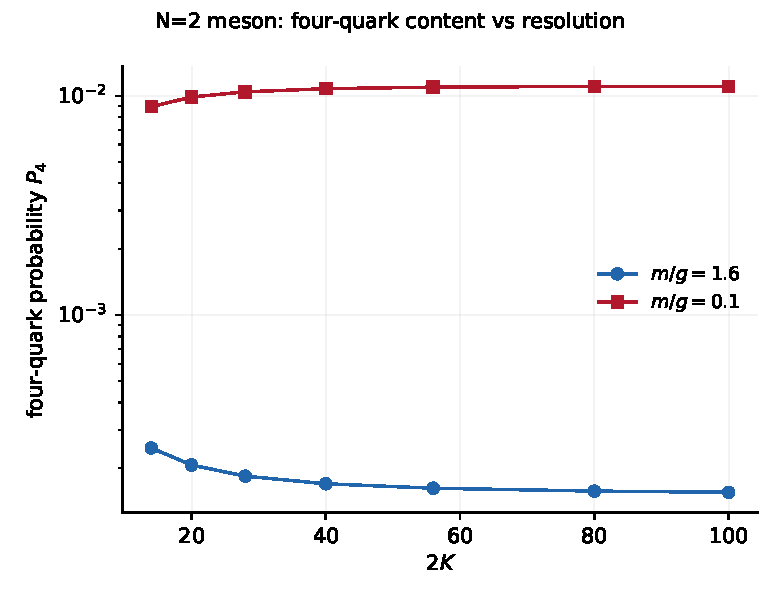
\includegraphics[width=0.8\columnwidth]{figs/fig22_p4_vs_K.pdf}
\caption{Four-quark probability $P_4$ of the $N=2$ meson ground state
against resolution, $m/g = 1.6$ and $0.1$, standard Hamiltonian,
$\mathrm{LPN} = 4$, no fits.  The published data reach $2K = 20$ (thesis
Fig.~22 of Ref.~\cite{Hornbostel:1988ne}); this extends the scan to
$2K = 100$.}
\label{fig:p4}
\end{figure}

One published measurement of this kind existed only in the thesis: the
$K$ dependence of higher-Fock content, at two resolutions.
Figure~\ref{fig:p4} extends it by a factor of five.  The two couplings
move in opposite directions.  At strong coupling the four-quark
probability grows with $K$ and saturates near one percent; at weak
coupling it falls toward a few parts in $10^4$.  Higher-Fock content is
not a fixed small number but a resolution-dependent one, and any
comparison of Fock truncations across $K$ inherits that dependence
(Appendix~\ref{app:budget}, the truncation component).
